\let\negmedspace\undefined
\let\negthickspace\undefined
\documentclass[journal]{IEEEtran}
\usepackage[a5paper, margin=10mm, onecolumn]{geometry}
%\usepackage{lmodern} % Ensure lmodern is loaded for pdflatex
\usepackage{tfrupee} % Include tfrupee package

\setlength{\headheight}{1cm} % Set the height of the header box
\setlength{\headsep}{0mm}     % Set the distance between the header box and the top of the text

\usepackage{gvv-book}
\usepackage{gvv}
\usepackage{cite}
\usepackage{amsmath,amssymb,amsfonts,amsthm}
\usepackage{algorithmic}
\usepackage{graphicx}
\usepackage{textcomp}
\usepackage{xcolor}
\usepackage{txfonts}
\usepackage{listings}
\usepackage{enumitem}
\usepackage{mathtools}
\usepackage{gensymb}
\usepackage{comment}
\usepackage[breaklinks=true]{hyperref}
\usepackage{tkz-euclide} 
\usepackage{listings}
% \usepackage{gvv}                                        
\def\inputGnumericTable{}                                 
\usepackage[latin1]{inputenc}                                
\usepackage{color}                                            
\usepackage{array}                                            
\usepackage{longtable}                                       
\usepackage{calc}                                             
\usepackage{multirow}                                         
\usepackage{hhline}                                           
\usepackage{ifthen}                                           
\usepackage{lscape}
\begin{document}

\bibliographystyle{IEEEtran}
\vspace{3cm}

\title{1-1.5-20}
\author{EE24BTECH11022 - Eshan Sharma
}
% \maketitle
% \newpage
% \bigskip
{\let\newpage\relax\maketitle}

\renewcommand{\thefigure}{\theenumi}
\renewcommand{\thetable}{\theenumi}
\setlength{\intextsep}{10pt} % Space between text and floats


\numberwithin{equation}{enumi}
\numberwithin{figure}{enumi}
\renewcommand{\thetable}{\theenumi}


\textbf{Question}:\\
Find the coordinates of a point $\vec{A}$ where AB is a diameter of the circle with centre $\brak{-2,2}$ and $\vec{B}$ is the point $\brak{3,4}$
\\
\textbf{Solution:}\\
Let the point $\vec{A}$ be $\brak{x,y}$.\\
Since AB is the diameter with centre of circle being $\brak{-2,2}$,\\
Centre of circle = $\frac{\vec{A}+\vec{B}}{2}$\\

\begin{align}
    \myvec{
        -2
        \\
        2
    }
    =
    \frac{1}{2} \brak{
    \myvec{
        x
        \\
        y
    }
    +
    \myvec{
        3
        \\
        4
    }
    }
\end{align}
\begin{align}
    \myvec{-2 \\ 2} &= \frac{1}{2} \left( \myvec{x \\ y} + \myvec{3 \\ 4} \right) \\
    2 \cdot \myvec{-2 \\ 2} &= \myvec{x \\ y} + \myvec{3 \\ 4} \\
    \myvec{-4 \\ 4} &= \myvec{x + 3 \\ y + 4} \\
    -4 &= x + 3 \\
    x &= -4 - 3 = -7 \\
    4 &= y + 4 \\
    y &= 4 - 4 = 0
\end{align}

Therefore, the coordinates of point $\vec{A}$ are $\boxed{(-7, 0)}$.

\begin{figure}[h]
    \centering
    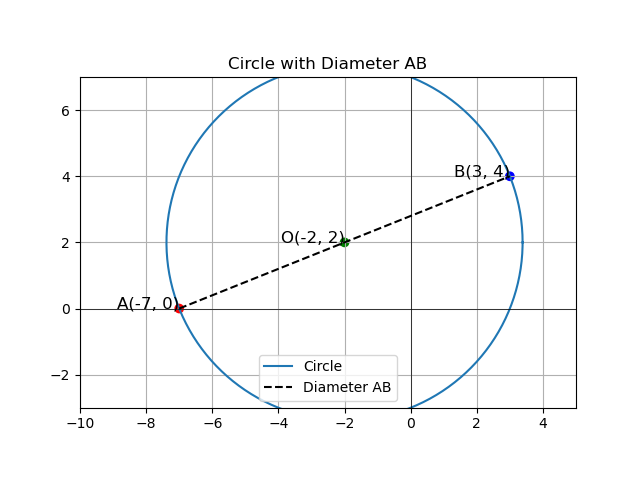
\includegraphics[width=0.6\textwidth]{circle_plot.png}
    \caption{Circle with Diameter \( AB \) and Center \( O(-2, 2) \)}
    \label{fig:circle_plot}
\end{figure}



\end{document}  
\end{document}
